\documentclass[12pt]{article}
\usepackage{graphicx}
\addtolength{\evensidemargin}{-0.5in}
\addtolength{\oddsidemargin}{-0.5in}
\addtolength{\textwidth}{1.0in}
%\input{math_macros.tex}
\def\half{{1\over 2}}
\begin{document}
\begin{center}
{\large\bf Some Comments on Likelihood Functions}
\end{center}
\vskip0.2in
The likelihood ${\cal L}$ is a function of the parameters of a statistical model.  It is
used to estimate the values of and uncertainties on those parameters for a given set of measurements.
For an ensemble of  $n$ measurements, the likelihood is defined as
$$
{\cal L}(x;\theta) = \prod_{i=1}^n {\cal L}_i(x;\theta) = \prod_{i=1}^n f(x;\theta)
$$
where $f(x;\theta)$ is the probability density function for the statistical model of interest.
The best value of the parameters $\theta$ can be determined by maximizing the likelihood function,
or equivalently, the log of the likelihood function.
\begin{eqnarray*}
  \frac{\partial \ln {\cal L}}{\partial  \theta} & = & 
  \frac{\partial} {\partial \theta} \ln \prod_{i=1}^n {\cal L}_i   \\
 & = & \frac{\partial}{\partial \theta} \sum_{i=1}^n \ln {\cal L}_i \\
 & = & 0 \\
\end{eqnarray*}
Often this procedure is described instead as minimizing $-\ln {\cal L}$ (minimizing the minus log likelihood).

The log likelihood can be Taylor expanded about its minimum.
Since $\partial {\cal L } /\partial \theta |_{\theta=\theta_{min}}=0$:
\begin{eqnarray*}
  \ln {\cal L} & = & \ln {\cal L}_{min} +\half \frac{\partial^2 \ln {\cal L}}{\partial \theta^2} \bigg|_{\theta=\theta_{min}}
  \left ( \theta -\theta_{min} \right )^2 \\
    2\left (\ln {\cal L} -\ln {\cal L}_{min} \right ) & = &  \frac{\partial^2 \ln {\cal L}}{\partial \theta^2} \bigg|_{\theta=\theta_{min}}
  \left ( \theta -\theta_{min} \right )^2 \\
\end{eqnarray*}
In the limit of large  $n$, the distribution ${\cal L}$  (due to the central limit theorem) becomes Gaussian.
Since for a Gaussian distribution
a change in $2\ln {\cal L}$ of one unit corresponds to a 1-$\sigma$ variation in
the parameter $\theta$,
the uncertainty on $\theta$ is given by:
$$
        {\sigma_\theta}^2 \equiv
        \left < \left ( \theta-\theta_{min} \right )^2 \right >  =  - \frac{1}{\frac{\partial^2 \ln {\cal L}}
  {\partial \theta^2}} \\
$$
Alternatively, the uncertainty
on the estimated values of the parameters $\theta$ can be obtained by calculating the value of
$\Delta \theta$  at which $-2\ln {\cal L}$ increases by 1.0.  In cases where $\ln {\cal L}$ is not
parabolic, the uncertainties can be asymmetric.

The definitions above depend on the fact that the probability density function $f(x;\theta)$ is normalized
over the region of $x$ where measurements can occur
$$
\int_{xmin}^{xmax} f(x;\theta) dx = 1
$$
For this reason, likelihood fits are not sensitive to the value of $n$.  It is possible to add a Poisson term
to the likelihood function to include the number of events in the likelihood fit.  When a fit includes
such a term, it is called
an {\it extended likelihood fit}.


\section*{An example}

Suppose a set of measurements $x_i$ are made in an experimental setup where the number of
events as a function of $x$ follows the distribution
$$
N(x) = A + Bx \;\;\; \mathrm{ for }\; 0<x<10 
$$
We would like to use the likelihood method to estimate the value of $\kappa \equiv A/B$.  Let's see how to
setup this problem.


The total number of events $N_{Tot}$ can be determined
\begin{eqnarray*}
  N_{Tot} & = & \int_0^{10} A+Bx \\
  & = & \left (Ax+\half B x^2 \right) \bigg|_0^{10} \\
  & = & 10A + \half (100B ) \\
  & = & 10A + 50B \\
\end{eqnarray*}
and  normalized probability density function $f(x;\theta)$ is
\begin{eqnarray*}
  f(x;A,B) & = & \frac{1}{N_{Tot}} \left ( A+Bx \right ) \\
  & = & \frac{1}{10A + 50B} \left ( A+Bx \right ) \\
  & = & \frac{A}{10A+50B} + \frac{Bx}{10A+50B} \\
  & = & 0.1 \left (\frac{\kappa}{\kappa+5} + \frac{x}{\kappa + 5} \right )\\
\end{eqnarray*}
The overall likelihood function is therefore
$$
{\cal L}(x;\kappa) = \prod_{i=1}^n 0.1 \left (\frac{\kappa}{\kappa+5} + \frac{x_i}{\kappa + 5} \right )\\
$$
and the log likelihood is
\begin{eqnarray*}
  \ln \left ( {\cal L}(x;\kappa)\right )  & = & 
  \sum_{i=1}^n \ln \left ( 0.1 \left (\frac{\kappa}{\kappa+5} + \frac{x_i}{\kappa + 5} \right ) \right )\\
  & = & 
    \sum_{i=1}^n \ln \left ( \left (\frac{\kappa}{\kappa+5} + \frac{x_i}{\kappa + 5} \right ) \right )
    + n\ln(0.1) \\
\end{eqnarray*}
If the values $x_i$ are known, then $-\ln \left ( {\cal L}(x;\kappa)\right )$ can be minimized with
respect to $\kappa$.  Because the last term in independent of $x_i$, it merely adds a constant term to the log likelihood
and is irrelevant for the minimization.

There are many programs available to do such minimization  However, it is sometimes useful to
start with the simplest approach.  It is possible to visualize the minimization process
by seeing how $\ln \left ( {\cal L}(x;\kappa)\right )$ changes when $\kappa$ is varied.  An example
root macro to generate fake data for the case $A=1$, $B=2$ and to use these data to determine
$\kappa$ can be found here:
\begin{flushleft}
http://physics.lbl.gov/shapiro/Physics226/myLikelihoodFit.C
\end{flushleft}
The output of this macro is provided on the next page:
\begin{figure}
\begin{center}
  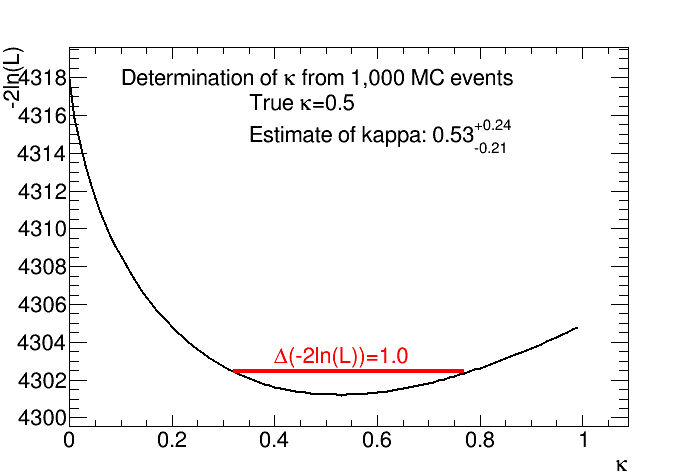
\includegraphics[width=8.0in]{lnLikelikhood.png}
\end{center}
\end{figure}
\end{document}
